\documentclass[11pt,a4paper]{article}

% ====== Gói ======
\usepackage{fontspec}          % font Unicode -> tiếng Việt gốc
\usepackage{amsmath,amssymb}
\usepackage{graphicx}
\usepackage{booktabs}
\usepackage{array}
\usepackage{multirow}
\usepackage{caption}
\usepackage{geometry}
\usepackage{hyperref}
\usepackage{xcolor}
\geometry{margin=2.5cm}
\hypersetup{colorlinks=true,linkcolor=blue,citecolor=blue,urlcolor=blue}

\renewcommand{\abstractname}{Tóm tắt}
\renewcommand{\tablename}{Bảng}
\renewcommand{\figurename}{Hình}
\renewcommand{\refname}{Tài liệu tham khảo}
\renewcommand{\contentsname}{Mục lục}

\captionsetup{font=small,labelfont=bf}
\newcommand{\R}{\textsc{Rescue}}
\newcommand{\wave}{\textsc{Wave}}

\title{\textbf{Máy học véc-tơ tựa song sinh dựa trên hạt hột với hàm mất mát bị chặn Wave và điều khiển theo độ thuần\\ \large (Purity-Adaptive Bounded-Loss Granular-Ball Twin SVM: PA-BL-GBTSVM)}}
\author{Nguyễn Trần Nguyệt Minh\\ \small Bản thảo, \today}
\date{}

\begin{document}
\maketitle

% ==================================================================
\begin{abstract}
\noindent
Nhiễu nhãn là thách thức cố hữu của phân loại có giám sát: các mẫu bị gán sai kéo mặt phân tách ra khỏi vị trí đúng, đặc biệt khi mô hình dùng hàm mất mát không bị chặn như hinge. Bài báo đề xuất \textbf{PA-BL-GBTSVM}, kết hợp ba thành phần: (i) biểu diễn dữ liệu bằng \emph{hạt hột} (granular ball) sinh theo ngưỡng độ thuần, giúp gộp nhiễu cục bộ và nén dữ liệu; (ii) thay hinge trong máy véc-tơ tựa song sinh trên hạt (GBTSVM) bằng \emph{hàm mất mát Wave bị chặn}, khả vi và tự triệt tiêu ảnh hưởng (redescending), giải bằng Adam; và (iii) cơ chế \emph{cứu suy biến} (rescue-only) kích hoạt theo điều kiện quan sát được khi một lớp mất hết hạt. Trên 10 bộ dữ liệu nhị phân với bốn kiểu nhiễu tổng hợp (đối xứng, bất đối xứng, biên, xa) và trên \emph{nhiễu nhãn thật} của CIFAR-10N, phương pháp cho thấy Wave trên hạt độ thuần cao vượt hinge một cách nhất quán, còn cơ chế cứu suy biến khôi phục các trường hợp mà GBTSVM và Wave-GBTSVM thuần bị hỏng, với độ lệch chuẩn nhỏ qua nhiều hạt giống ngẫu nhiên. Cơ chế cứu chỉ dựa trên một dấu hiệu \emph{đo được} (một lớp còn dưới ngưỡng số hạt), nên triển khai được trên dữ liệu thật mà không cần biết trước cấu trúc nhiễu.

\medskip
\noindent\textbf{Từ khóa:} nhiễu nhãn, hàm mất mát bị chặn, hạt hột, máy véc-tơ tựa song sinh, độ thuần, suy biến lớp.
\end{abstract}

% ==================================================================
\section{Giới thiệu}
\label{sec:intro}

Trong phân loại có giám sát, chất lượng nhãn quyết định phần lớn chất lượng mô hình. Tuy nhiên nhãn thực tế thường chứa \emph{nhiễu}: sai sót của người gán, quy tắc gán mơ hồ ở vùng biên, hoặc dữ liệu gán tự động. Nhiễu nhãn làm lệch mặt phân tách và giảm khả năng khái quát, nhất là với các mô hình biên cứng dùng hàm mất mát \emph{không bị chặn} như hinge: một mẫu bị gán sai nằm sâu trong lớp đối phương tạo vi phạm lớn và bị phạt tuyến tính không giới hạn, kéo siêu phẳng về phía nó \cite{frenay2014}.

Hai hướng khắc phục bổ sung cho nhau. Thứ nhất, \emph{hàm mất mát bị chặn} (bounded loss) giới hạn mức phạt tối đa mà một mẫu có thể gây ra; hàm Wave gần đây \cite{wave2024} vừa bị chặn, vừa trơn và \emph{tự triệt tiêu} (redescending): mẫu càng bất thường thì đạo hàm càng về 0, nên ảnh hưởng của ngoại lai bị dập tắt thay vì khuếch đại. Thứ hai, \emph{học trên hạt hột} (granular-ball learning) \cite{xia2019} thay mỗi vùng dữ liệu cùng nhãn bằng một quả bóng đặc trưng bởi tâm và bán kính; việc lấy trung bình cục bộ vừa nén dữ liệu, vừa làm loãng các nhãn sai lẻ tẻ.

Máy véc-tơ tựa song sinh (Twin SVM) \cite{tsvm2007} học hai siêu phẳng không song song, mỗi cái gần một lớp và cách xa lớp còn lại, cho lời giải nhanh hơn SVM chuẩn. Phiên bản trên hạt, gọi là GBTSVM, áp Twin SVM lên tâm và bán kính của các hạt. Bài báo này ghép \emph{ba} ý tưởng: hạt hột (điều khiển bằng ngưỡng độ thuần), hàm Wave bị chặn, và Twin SVM, đồng thời giải quyết một hệ quả thực tế của việc gộp hạt dưới nhiễu: hiện tượng \emph{suy biến mất lớp}, khi một lớp không còn hạt nào và bài toán song sinh sụp đổ.

\paragraph{Đóng góp.} Cụ thể, bài báo:
\begin{enumerate}
\item Đề xuất \textbf{Wave-GBTSVM}: thay hinge trong GBTSVM bằng hàm mất mát Wave bị chặn áp \emph{trên hạt}, biến hai bài toán con thành tối ưu không ràng buộc trơn, giải bằng Adam (Mục~\ref{sec:method}).
\item Phân tích lý do áp hàm bị chặn \emph{lên hạt} hiệu quả hơn lên từng điểm, dựa trên tính trung bình cục bộ của tâm hạt (Mục~\ref{sec:why}).
\item Đề xuất cơ chế \emph{cứu suy biến} \R{}-only kích hoạt theo điều kiện quan sát được (một lớp còn dưới ngưỡng số hạt), khôi phục các lát cắt bị hỏng mà gần như không tốn thêm hạt (Mục~\ref{sec:rescue}).
\item Kiểm chứng trên bốn kiểu nhiễu tổng hợp và trên \emph{nhiễu nhãn thật} CIFAR-10N, kèm khảo sát cắt bỏ (ablation) về ngưỡng kích hoạt và độ nén (Mục~\ref{sec:exp} và~\ref{sec:results}).
\end{enumerate}

% ==================================================================
\section{Kiến thức nền và công trình liên quan}
\label{sec:background}

\subsection{Máy véc-tơ tựa song sinh trên hạt (GBTSVM)}
Cho tập huấn luyện nhị phân, hạt hột chia dữ liệu thành các quả bóng, mỗi bóng $B_k$ có tâm $c_k\in\mathbb{R}^d$, bán kính $r_k\ge 0$ và nhãn đa số $y_k\in\{+1,-1\}$. GBTSVM tìm hai siêu phẳng $f_+(x)=w_+^\top x + b_+$ và $f_-(x)=w_-^\top x + b_-$: siêu phẳng $+$ bám các tâm bóng lớp $+1$ và đẩy các bóng lớp $-1$ (đã cộng bán kính) qua lề, và ngược lại. Với hinge, mỗi bài toán con là một quy hoạch toàn phương (QP) có ràng buộc, giải bằng bộ giải QP. Một mẫu mới $x$ được gán nhãn theo siêu phẳng gần nó hơn:
\begin{equation}
\hat{y}(x) = \operatorname*{arg\,min}_{s\in\{+,-\}} \frac{|f_s(x)|}{\|w_s\|}.
\end{equation}

\subsection{Hàm mất mát Wave}
Hàm Wave \cite{wave2024} với tham số hình dạng $a>0$ và tham số trần $\lambda>0$ được định nghĩa
\begin{equation}
\label{eq:wave}
L(u;\lambda,a) \;=\; \frac{1}{\lambda}\!\left(1 - \frac{1}{1+\lambda\,u^{2}e^{a u}}\right)
\;=\; \frac{u^{2}e^{a u}}{1+\lambda\,u^{2}e^{a u}},
\end{equation}
trong đó $u$ là độ vi phạm lề. Hàm này (i) \emph{bị chặn} bởi $1/\lambda$, nên một mẫu dù bất thường đến đâu cũng chỉ đóng góp mức phạt tối đa $1/\lambda$; (ii) \emph{trơn}, nên bài toán khả vi và giải được bằng gradient; và (iii) \emph{tự triệt tiêu}: khi $u$ lớn, $L\to 1/\lambda$ và $L'\to 0$, tức ngoại lai không còn kéo được siêu phẳng. Với $u$ nhỏ, $L(u)\approx u^2 e^{au}$ độc lập với $\lambda$, nên $\lambda$ chỉ đặt \emph{trần bão hòa} chứ không đổi hành vi ở vùng gần lề.

% ==================================================================
\section{Phương pháp đề xuất}
\label{sec:method}

\subsection{Sinh hạt theo ngưỡng độ thuần}
\label{sec:balls}
Từ tập điểm, ta sinh hạt bằng cách chia đệ quy: một bóng được tách làm hai bằng 2-means khi \emph{độ thuần} của nó
\begin{equation}
p_k = \frac{\#\{\text{điểm thuộc lớp đa số trong } B_k\}}{|B_k|}
\end{equation}
còn nhỏ hơn ngưỡng $\rho$, và dừng khi $p_k \ge \rho$ hoặc bóng chỉ còn một điểm. Tâm $c_k$ là trung bình các điểm trong bóng, bán kính $r_k$ là khoảng cách trung bình từ các điểm tới tâm, nhãn $y_k$ là nhãn đa số. Ngưỡng $\rho$ điều tiết đánh đổi: $\rho=1$ buộc mọi bóng thuần tuyệt đối (nén yếu, nhiều bóng nhỏ), $\rho<1$ cho phép bóng lẫn (nén mạnh, gộp nhiễu vào trung bình cục bộ).

\subsection{Wave-GBTSVM}
\label{sec:wavegb}
Ta thay hinge trong GBTSVM bằng hàm Wave~\eqref{eq:wave} áp trên hạt. Ký hiệu $H_+$ là ma trận $[C_+\;\mathbf{1}]$ của các bóng lớp $+1$ (tương tự $H_-$), và $z_+=[w_+;b_+]$. Siêu phẳng $+$ giải bài toán \emph{không ràng buộc}:
\begin{equation}
\label{eq:obj}
\min_{z_+}\;\; \tfrac{1}{2}\,\|H_+ z_+\|^2 \;+\; \tfrac{1}{2}\,\varepsilon\,\|z_+\|^2 \;+\; c\!\!\sum_{k:\,y_k=-1}\!\! L\!\big(1 + r_k + (H_k^{-} z_+);\,\lambda_k,\,a\big),
\end{equation}
trong đó số hạng thứ nhất kéo siêu phẳng bám tâm bóng cùng lớp, số hạng $\varepsilon$ là điều hòa Tikhonov, và số hạng Wave phạt các bóng đối phương vi phạm lề $u_k = 1 + r_k + (H_k^{-}z_+)$; cộng $r_k$ nghĩa là dùng \emph{mép} bóng thay vì tâm. Siêu phẳng $-$ đối xứng. Vì Wave trơn, ta không cần QP hay nghịch đảo $(A^\top A)^{-1}$; mỗi bài toán con giải bằng Adam \cite{adam2015}. Trần $\lambda_k$ có thể là hằng dùng chung ($\lambda_k\equiv\lambda_0$), hoặc điều biến theo độ thuần từng bóng (xem Mục~\ref{sec:discussion}). Trong cấu hình chính của bài báo, ta dùng $\lambda_k\equiv\lambda_0$ cố định vì nó đơn giản và đã đủ mạnh.

\subsection{Cơ chế cứu suy biến (rescue-only)}
\label{sec:rescue}
Khi $\rho<1$ và nhiễu \emph{bất đối xứng} (một lớp bị lật nhiều hơn), việc gộp hạt có thể khiến \emph{toàn bộ} hạt của một lớp bị gán nhãn đa số về lớp kia; lúc đó lớp đó không còn hạt nào và bài toán song sinh~\eqref{eq:obj} \emph{suy biến} (không có mặt để khớp). Ta đề xuất cơ chế cứu \emph{tối thiểu}: khi một lớp $c$ còn dưới $\text{floor}$ hạt, với mỗi bóng đang chứa điểm nhãn $c$ (dù là thiểu số), ta bổ sung một bóng con lấy \emph{tâm của cụm điểm nhãn $c$} bên trong bóng đó, gán nhãn $c$. Với $\text{floor}=1$, cơ chế chỉ ra tay khi một lớp \emph{đã cạn hoàn toàn}. Điểm mấu chốt: điều kiện kích hoạt là \emph{đo được} (đếm số hạt mỗi lớp), không cần biết trước loại nhiễu, nên áp dụng được trên dữ liệu thật.

Tuy nhiên, ở chế độ sụp cực đoan, sau khi cứu một lớp thường chỉ còn \emph{một} hạt (Mục~\ref{sec:nc}). Khi một lớp chỉ có một tâm, hai mặt phẳng song sinh mất ý nghĩa lề vì một điểm không định được hướng siêu phẳng. Do đó ta bổ sung một quy tắc \emph{thoái lui}: khi một lớp còn $\le 1$ hạt, thay vì cố khớp twin-SVM, mô hình chuyển sang quyết định \emph{nearest-centroid} (gán mẫu theo tâm hạt gần nhất). Với một tâm dương và một tâm âm, nearest-centroid chính là đường trung trực giữa hai tâm, một ranh giới ổn định và hợp lý hơn twin-SVM trong tình huống đó (bằng chứng ở Mục~\ref{sec:nc}). Ngưỡng thoái lui ($\le 1$ hạt) là một siêu tham số có thể tinh chỉnh, bàn ở Mục~\ref{sec:discussion}.

Hình~\ref{fig:svmgb} minh họa vì sao áp hàm bị chặn lên hạt lợi hơn lên điểm, và Hình~\ref{fig:twocent} minh họa cơ chế hai-tâm dùng trong bước cứu.

\begin{figure}[t]
\centering
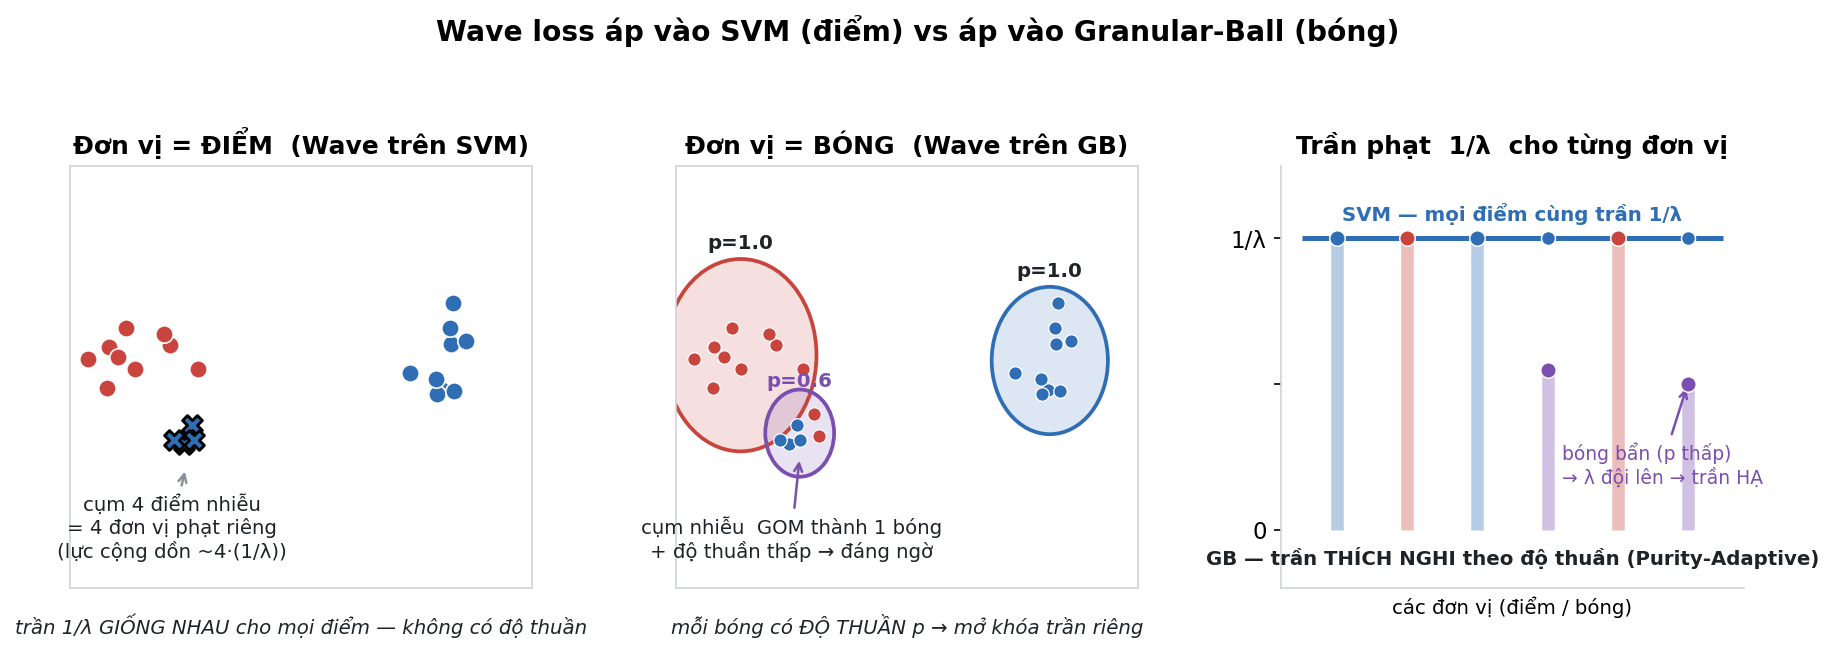
\includegraphics[width=0.9\linewidth]{svm_vs_gb.png}
\caption{Áp hàm mất mát bị chặn lên \emph{điểm} (trái) so với lên \emph{hạt} (phải). Tâm hạt là trung bình cục bộ nên nhãn sai lẻ tẻ bị làm loãng trước khi vào hàm mất mát; số bóng sai nhãn ít và bị Wave tự triệt tiêu, trong khi từng điểm nhiễu vẫn kéo được biên.}
\label{fig:svmgb}
\end{figure}

\begin{figure}[t]
\centering
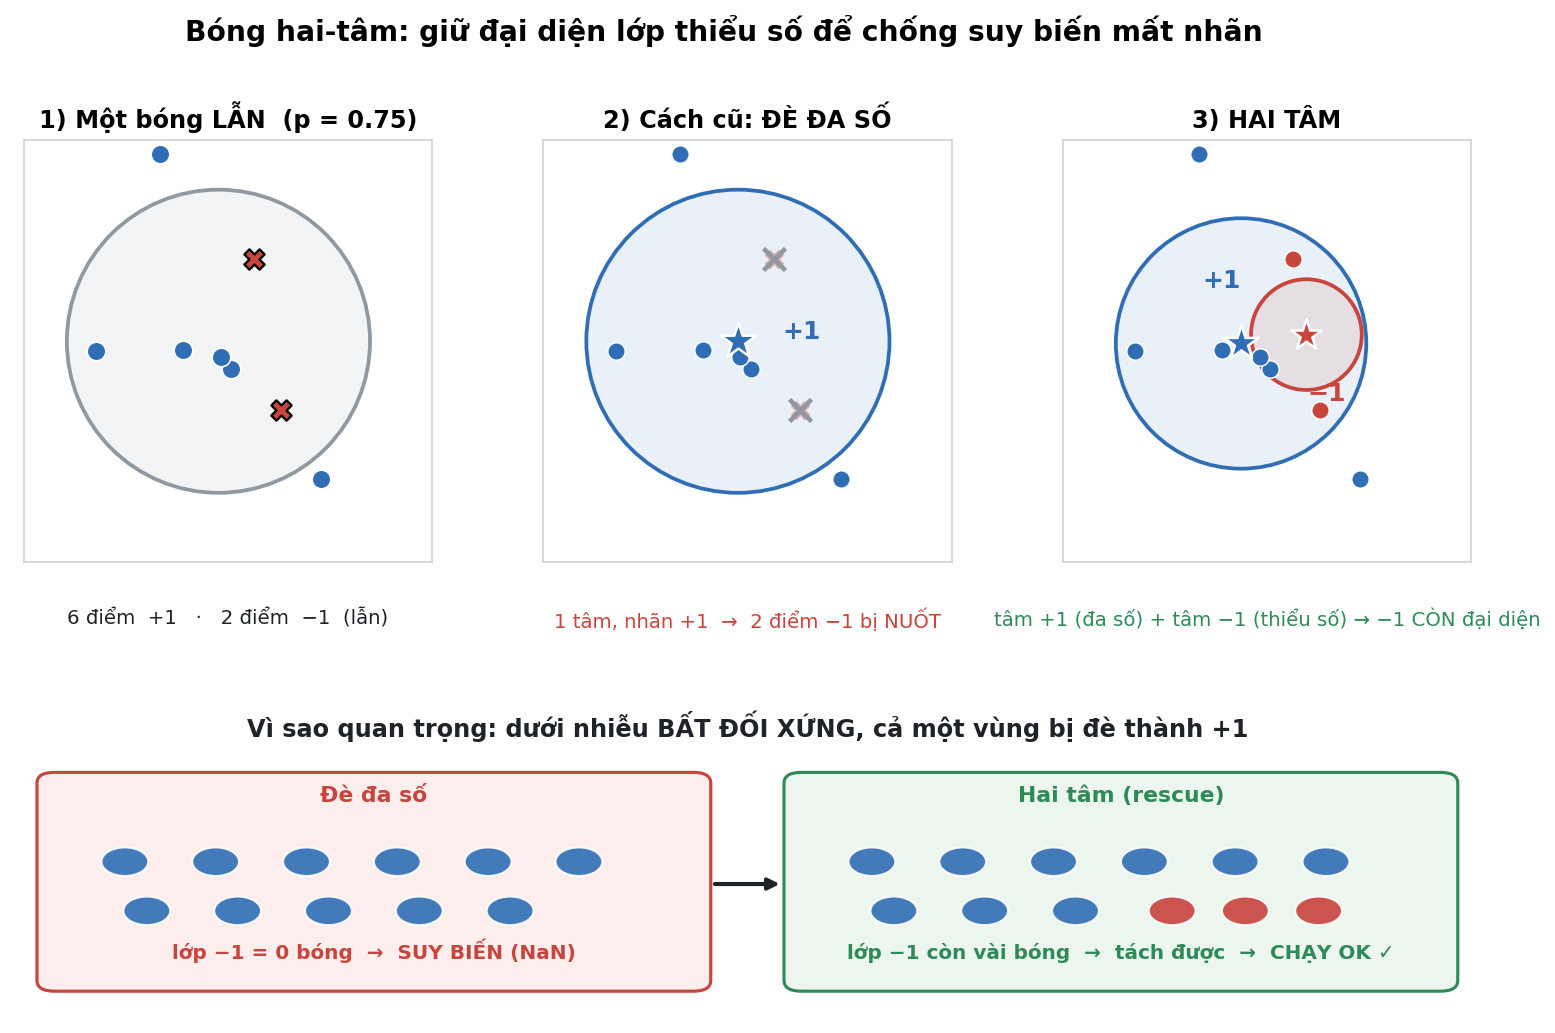
\includegraphics[width=0.72\linewidth]{twocent.png}
\caption{Cơ chế hai-tâm dùng trong bước cứu: một bóng lẫn được bổ sung tâm của cụm điểm lớp thiểu số để bảo toàn đại diện cho lớp sắp mất, tránh suy biến song sinh.}
\label{fig:twocent}
\end{figure}

% ==================================================================
\section{Vì sao ghép Wave với hạt, không phải với SVM điểm}
\label{sec:why}
Áp hàm Wave lên \emph{từng điểm} vẫn chặn được mức phạt của mỗi điểm, nhưng mỗi điểm nhiễu vẫn là một số hạng riêng kéo siêu phẳng. Áp lên \emph{hạt} có hai lợi ích cộng dồn. Thứ nhất, tâm bóng là trung bình cục bộ: dưới nhiễu vừa phải, đa số điểm trong bóng đúng nhãn nên tâm nằm đúng phía, và ảnh hưởng của vài điểm sai đã bị pha loãng \emph{trước khi} vào hàm mất mát. Thứ hai, số hạt sai nhãn (bóng có nhãn đa số sai) ít hơn nhiều so với số điểm sai nhãn, và mỗi bóng như vậy chỉ đóng góp tối đa $1/\lambda$ rồi bị đạo hàm triệt tiêu. Nói cách khác, hạt lọc nhiễu ở mức \emph{biểu diễn}, Wave chặn nhiễu ở mức \emph{mục tiêu}; hai lớp phòng vệ nối tiếp nhau.

% ==================================================================
\section{Thiết lập thực nghiệm}
\label{sec:exp}

\paragraph{Bộ dữ liệu.} Mười bộ nhị phân chuẩn: \textit{balance\_scale, breast\_cancer, SPECTF, haberman, heart, ionosphere, sonar, banknote, australian, german}. Mỗi bộ chuẩn hóa về $[-1,1]$ và đánh giá bằng kiểm định chéo 5 lớp phân tầng.

\paragraph{Kiểu nhiễu tổng hợp.} Bốn kiểu, mỗi kiểu ở các mức tỉ lệ $\{0.2,0.3,0.4,0.5\}$: \emph{đối xứng} (lật ngẫu nhiên hai chiều), \emph{bất đối xứng} (chỉ lật một lớp, gây mất cân bằng nhãn nhiễu), \emph{biên} (lật các điểm gần mặt phân tách), \emph{xa} (lật các điểm xa tâm lớp). Nhiễu chỉ tiêm vào tập huấn luyện; tập kiểm tra giữ nhãn sạch.

\paragraph{Nhiễu nhãn thật.} CIFAR-10N \cite{cifar10n} cung cấp nhãn do người gán (nhiễu thật) kèm nhãn sạch cho CIFAR-10. Ta dựng bài nhị phân tabular: chọn hai lớp, trích đặc trưng ảnh phẳng $\to$ chuẩn hóa $\to$ PCA $\to$ MinMax$(-1,1)$; nhãn huấn luyện là nhãn-người (chiếu về nhị phân, lớp thứ ba coi là lật), nhãn kiểm tra là nhãn sạch.

\paragraph{Mô hình và cấu hình.} GBTSVM (hinge, QP) làm chuẩn so; Wave-GBTSVM với $c_1=c_2=10$, $\lambda_0=1$, $a=1$, $\varepsilon=10^{-3}$, Adam $250$ bước. Bóng sinh với ngưỡng $\rho$ nêu trong từng thí nghiệm. Chỉ số chính là độ chính xác trên tập kiểm tra sạch, trung bình trên 5 hạt giống ngẫu nhiên (báo cáo kèm độ lệch chuẩn).

% ==================================================================
\section{Kết quả và thảo luận}
\label{sec:results}

\subsection{Độ chính xác trên nhiễu tổng hợp}
Bảng~\ref{tab:synth} tổng hợp độ chính xác trung bình trên toàn giao thức nhiễu (bốn kiểu $\times$ các mức $0.2$ đến $0.5$, 10 bộ, 5 hạt giống). Ở độ thuần cao ($\rho=1$), Wave vượt hinge nhất quán ($0.702$ so với $0.687$). Ở độ thuần thấp, cơ chế cứu nâng thêm độ chính xác so với cả hai đường cơ sở.

\begin{table}[h]
\centering
\caption{Độ chính xác trung bình trên giao thức nhiễu tổng hợp (10 bộ, 5 hạt giống, nhân tuyến tính).}
\label{tab:synth}
\begin{tabular}{lccc}
\toprule
Độ thuần $\rho$ & GBTSVM (hinge) & Wave-GBTSVM & Wave + \R{} \\
\midrule
$\rho=1.0$ & $0.687$ & $\mathbf{0.702}$ & \\
$\rho=0.7$ & $0.647$ & $0.652$ & $\mathbf{0.662}$ \\
$\rho=0.6$ & $0.655$ & $0.657$ & $\mathbf{0.667}$ \\
\bottomrule
\end{tabular}
\end{table}

\subsection{Độ nén (số hạt so với số điểm)}
Bảng~\ref{tab:comp} cho thấy độ thuần thấp nén mạnh hơn nhiều. Ở $\rho=1$ số bóng gần bằng số điểm (nén $1.4$ đến $2.1\times$, kém) vì dưới nhiễu, để đạt thuần tuyệt đối phần lớn bóng bị tách tới mức đơn lẻ. Ở $\rho=0.7$ nén $3.6$ đến $9.4\times$, ở $\rho=0.6$ nén tới $32$ đến $116\times$. Quan trọng: cơ chế cứu chỉ thêm khoảng $0$ đến $1$ bóng, nên gần như không ảnh hưởng độ nén.

\begin{table}[h]
\centering
\caption{Độ nén (số điểm / số bóng) theo ngưỡng độ thuần; cơ chế cứu thêm $\sim 0$ đến $1$ bóng.}
\label{tab:comp}
\begin{tabular}{lc}
\toprule
Độ thuần $\rho$ & Độ nén (điểm/bóng) \\
\midrule
$\rho=1.0$ & $1.4$ đến $2.1\times$ \\
$\rho=0.7$ & $3.6$ đến $9.4\times$ \\
$\rho=0.6$ & $32$ đến $116\times$ \\
\bottomrule
\end{tabular}
\end{table}

\subsection{Chống suy biến và các khảo sát cắt bỏ}
\label{sec:ablation}
Cơ chế cứu $\R$-only ($\text{floor}=1$) khôi phục các lát cắt bị suy biến dưới nhiễu bất đối xứng mà không làm hại các trường hợp khác. Ta khảo sát hai lựa chọn thay thế và thấy đều không tốt hơn:
\begin{itemize}
\item \textbf{Kích hoạt sớm (quét floor).} Với $\text{floor}\in\{1,5,10,20\}$, độ chính xác gần như bằng nhau ($\approx 0.625$); $\text{floor}=1$ là tối ưu, kích hoạt sớm không thêm lợi. Vậy nên chỉ cứu khi lớp \emph{thật sự} cạn hạt.
\item \textbf{Tách chủ động theo ngưỡng $\tau$.} Nếu tách mọi bóng lẫn có độ thuần dưới $\tau$ (thay vì chỉ cứu khi suy biến), độ chính xác giúp nhiễu bất đối xứng ($+0.01$) nhưng \emph{hại} các kiểu đối xứng/biên/xa ($-0.04$ đến $-0.08$); phương án chỉ cứu ($\tau=0.7$) cho tổng thể tốt nhất ($0.625$). Tách chủ động cần biết trước nhiễu là bất đối xứng nên không triển khai được; cơ chế cứu \emph{phản ứng} mới đúng.
\item \textbf{Hạt bền (robust ball).} Thay tâm/bán kính bằng thống kê bền với ngoại lai chỉ tăng $0.003$, không đáng, nên loại.
\end{itemize}

\subsection{Tự dò siêu tham số (tiện ích)}
Với nhân RBF, dò $\lambda,C,\gamma$ bằng thuật toán bầy đàn (WOA/PSO) so với lưới thô cho kết quả trái chiều nhưng \emph{ổn định} hơn: trên \textit{sonar} $+0.081$, \textit{ionosphere} $+0.155$, \textit{heart} $-0.056$; lưới RBF thỉnh thoảng sụp gần mức ngẫu nhiên do $\gamma$ thô, còn dò liên tục hiếm khi sụp, đổi lại tốn khoảng $6\times$ số lần chấm. Ta xem đây là tiện ích tự dò cho RBF, không phải đóng góp chính.

\subsection{Nhiễu nhãn thật (CIFAR-10N)}
\label{sec:realnoise}
Bảng~\ref{tab:real} báo cáo cặp \textit{automobile} vs \textit{truck} (nhiễu thật $7.6\%$, PCA $100$ chiều), trung bình $\pm$ độ lệch chuẩn trên 5 hạt giống. Hai kết luận vững:
\emph{(i)} Wave$(\rho{=}1)$ đạt $0.704\pm 0.004$, nhỉnh hơn hinge$(\rho{=}1)$ $0.696\pm 0.003$ một cách nhất quán qua cả 5 hạt giống với độ lệch chuẩn nhỏ.
\emph{(ii)} Ở $\rho=0.5$, cả GBTSVM và Wave-GBTSVM thuần đều \emph{suy biến trên toàn bộ 5 hạt giống} (một lớp mất sạch hạt), trong khi Wave $+$ \R{} khôi phục về $0.656\pm 0.002$. Đây là bằng chứng cơ chế cứu hoạt động trên nhãn nhiễu \emph{thật}, ổn định qua nhiều hạt giống.

\begin{table}[h]
\centering
\caption{Nhiễu nhãn thật CIFAR-10N, \textit{automobile} vs \textit{truck} (nhiễu $7.6\%$, PCA $100$), độ chính xác trên test sạch, trung bình $\pm$ độ lệch chuẩn trên 5 hạt giống. ``suy biến'' = cả 5 hạt giống mất hết hạt một lớp.}
\label{tab:real}
\begin{tabular}{lccccc}
\toprule
$\rho$ & hinge$(\rho{=}1)$ & Wave$(\rho{=}1)$ & hinge$(\rho)$ & Wave$(\rho)$ & Wave$+\R{}(\rho)$ \\
\midrule
$0.7$ & $0.696{\pm}.003$ & $\mathbf{0.704{\pm}.004}$ & $0.671{\pm}.007$ & $0.671{\pm}.009$ & $0.671{\pm}.009$ \\
$0.5$ & $0.696{\pm}.003$ & $\mathbf{0.704{\pm}.004}$ & suy biến & suy biến & $\mathbf{0.656{\pm}.002}$ \\
\bottomrule
\end{tabular}
\end{table}

Cặp khó \textit{cat} vs \textit{dog} (nhiễu thật $46.6\%$, PCA $50$) cho cả ba mô hình quanh $0.52$, sát mức đoán ngẫu nhiên: không gian đặc trưng PCA thấp mang quá ít tín hiệu để phân biệt phương pháp, nên ta chỉ dùng cặp này như minh họa giới hạn của đặc trưng, không phải bằng chứng chống lại phương pháp.

\subsection{SVM so với nearest-centroid: máy lề đáng giá ở đâu}
\label{sec:nc}
Một câu hỏi nền tảng: khi số hạt tụt xuống rất ít, liệu twin-SVM còn thực sự dùng đến \emph{lề}, hay đã suy về nearest-centroid (1-NN trên tâm hạt)? Để trả lời, ta so twin-SVM (wave và hinge) với nearest-centroid trên \emph{cùng một tập tâm hạt}, ở hai chế độ đối lập.

\emph{Ở độ thuần cao} ($\rho=1$, trung bình $\approx 188$ hạt), Bảng~\ref{tab:nc} cho thấy Wave vượt nearest-centroid $+0.080$ và thắng trên mọi bộ. Nhiều hạt thuần cho phép máy lề dựng một ranh giới toàn cục tốt hơn hẳn quyết định cục bộ theo tâm gần nhất. Đây là bằng chứng trực tiếp rằng ở chế độ chính, phần SVM \emph{đóng góp thật}, không phải kNN trá hình.

\emph{Ở độ thuần thấp} ($\rho=0.6$, sáu bộ, nhiễu đối xứng và bất đối xứng), bức tranh đảo ngược. Có tới $52\%$ số lát cắt \emph{sụp} về đúng một hạt mỗi lớp; ở các lát cắt này nearest-centroid đạt $0.784$ so với twin-SVM $0.716$. Ngay cả khi không sụp, ở $\rho=0.6$ nearest-centroid vẫn ngang hoặc nhỉnh hơn Wave. Tức ở độ thuần thấp, không gian đã thuộc về nearest-centroid; twin-SVM không còn thêm giá trị. Điều này biện minh cho quy tắc thoái lui ở Mục~\ref{sec:rescue}: chuyển sang nearest-centroid khi một lớp còn $\le 1$ hạt nâng độ chính xác các lát cắt sụp từ $0.716$ lên $0.784$.

\begin{table}[h]
\centering
\caption{$\rho=1$: twin-SVM (hinge/Wave) so với nearest-centroid trên cùng tâm hạt (trung bình nhiễu đối xứng và bất đối xứng). Wave vượt nearest-centroid trên mọi bộ.}
\label{tab:nc}
\begin{tabular}{lcccc}
\toprule
bộ & số hạt & hinge & Wave & nearest-centroid \\
\midrule
breast\_cancer & $244$ & $0.772$ & $\mathbf{0.831}$ & $0.720$ \\
haberman & $183$ & $0.622$ & $0.614$ & $0.532$ \\
heart & $161$ & $0.679$ & $\mathbf{0.690}$ & $0.618$ \\
ionosphere & $163$ & $0.726$ & $\mathbf{0.741}$ & $0.686$ \\
\midrule
Trung bình & $188$ & $0.700$ & $\mathbf{0.719}$ & $0.639$ \\
\bottomrule
\end{tabular}
\end{table}

% ==================================================================
\section{Thảo luận}
\label{sec:discussion}
\paragraph{Định vị đóng góp.} Phương pháp chính, tức Wave bị chặn áp trên hạt độ thuần cao, \emph{không phụ thuộc loại nhiễu} và là tuyên bố trọng tâm; ở đó máy lề đóng góp thật, vượt cả hinge lẫn nearest-centroid (Mục~\ref{sec:nc}). Cơ chế cứu là mở rộng thứ cấp, kích hoạt theo dấu hiệu quan sát được nên khả triển khai; ta định vị nó một cách trung thực là cơ chế \emph{suy biến có kiểm soát} chứ không phải một chiến thắng của SVM: khi độ thuần thấp và một lớp cạn hạt, mô hình thoái lui về nearest-centroid, vì ở chế độ đó twin-SVM trên một vài tâm đã mất ý nghĩa lề và thua chính nearest-centroid.

\paragraph{Về biến thể $\lambda$ theo độ thuần.} Ta có khảo sát điều biến trần $\lambda_k$ theo độ thuần từng bóng, dạng $\lambda_k=\lambda_0(1+\kappa\,(1-p_k))$ (bóng càng lẫn thì trần càng thấp). Đây là một \emph{quy tắc thực nghiệm} do nhóm đề xuất, \emph{không} lấy từ công trình gốc về hàm Wave. Trong thực nghiệm, biến thể này không vượt trội rõ so với $\lambda$ cố định, nên ta chọn $\lambda$ cố định ($\kappa=0$) cho cấu hình chính và để biến thể thích nghi ở phần thảo luận/hướng phát triển.

\paragraph{Hướng phát triển.} Ngưỡng thoái lui về nearest-centroid hiện đặt ở mức một lớp còn $\le 1$ hạt, là lằn ranh tự nhiên (một hạt không dựng được lề). Có thể quét ngưỡng theo số hạt tối thiểu mỗi lớp để tìm chính xác điểm giao nơi twin-SVM bắt đầu vượt nearest-centroid, từ đó chọn mốc chuyển tối ưu thay vì mốc cố định; đây là một hướng tinh chỉnh để lại cho công việc sau. Ngoài ra, biến thể trần $\lambda_k$ thích nghi theo độ thuần (nêu trên) cũng là một nhánh mở.

\paragraph{Hạn chế.} Đặc trưng ảnh nén bằng PCA tuyến tính là không gian yếu cho phân loại tuyến tính; các cặp lớp khó (như cat/dog) không đủ tín hiệu để phân biệt phương pháp. Ngoài ra, hàm Wave giải bằng Adam nên phụ thuộc số bước và bước học, dù trong khảo sát của ta độ lệch chuẩn qua các hạt giống nhỏ.

% ==================================================================
\section{Kết luận}
\label{sec:conclusion}
Bài báo đề xuất PA-BL-GBTSVM, ghép biểu diễn hạt hột điều khiển theo độ thuần, hàm mất mát Wave bị chặn áp trên hạt, và cơ chế cứu suy biến kích hoạt theo điều kiện quan sát được. Trên nhiễu tổng hợp và nhiễu nhãn thật CIFAR-10N, Wave trên hạt độ thuần cao vượt hinge một cách nhất quán, và cơ chế cứu khôi phục các trường hợp suy biến với chi phí gần như bằng không về số hạt, độ lệch chuẩn nhỏ qua nhiều hạt giống. Hướng phát triển gồm: mở rộng đa lớp, đặc trưng phi tuyến mạnh hơn cho ảnh, và phân tích lý thuyết về điều kiện suy biến cùng cận sai số của bước cứu.

% ==================================================================
\begin{thebibliography}{9}
\bibitem{wave2024} M.~A. Akhtar, M.~Tanveer, and M.~Arshad, ``Wave loss: A novel bounded, smooth and asymmetric loss function for robust learning,'' \emph{Pattern Recognition}, 2024.
\bibitem{tsvm2007} Jayadeva, R.~Khemchandani, and S.~Chandra, ``Twin support vector machines for pattern classification,'' \emph{IEEE Trans. Pattern Anal. Mach. Intell.}, vol.~29, no.~5, 2007.
\bibitem{xia2019} S.~Xia, Y.~Liu, X.~Ding, G.~Wang, H.~Yu, and Y.~Luo, ``Granular ball computing classifiers for efficient, scalable and robust learning,'' \emph{Information Sciences}, 2019.
\bibitem{frenay2014} B.~Fr\'enay and M.~Verleysen, ``Classification in the presence of label noise: A survey,'' \emph{IEEE Trans. Neural Netw. Learn. Syst.}, vol.~25, no.~5, 2014.
\bibitem{cifar10n} J.~Wei, Z.~Zhu, H.~Cheng, T.~Liu, G.~Niu, and Y.~Liu, ``Learning with noisy labels revisited: A study using real-world human annotations,'' in \emph{ICLR}, 2022.
\bibitem{adam2015} D.~P. Kingma and J.~Ba, ``Adam: A method for stochastic optimization,'' in \emph{ICLR}, 2015.
\end{thebibliography}

\end{document}
